\documentclass[12pt,openright,twoside,a4paper,brazil]{abntex2}
\usepackage[utf8]{inputenc}
\usepackage[T1]{fontenc}
\usepackage{graphicx}
\usepackage{listing}
\usepackage{amsfonts}

\title{Projeto Interativo III - Angry Robots}
\date{}
\author{\textbf{Caroline Bomfim Do Espirito Santo} (caroline.bomfim@hotmail.com.br), \\ \textbf{Mahaira Soares de Souza} (mahaira\_souza@hotmail.com), \\ \textbf{Rafael da Silva Santos} (rafa\_silva.santos@hotmail.com), \\ \textbf{Thiago de Sousa Messias} (messiasthi@gmail.com). \\ \\ Ciência da Computação - Centro Universitário Senac}

\setlength{\parskip}{0.2cm} 
\setlrmarginsandblock{3cm}{2cm}{*}
\setulmarginsandblock{3cm}{2cm}{*}
\checkandfixthelayout

\begin{document}

\maketitle
 
\section*{Resumo}

Angry Robots é um jogo desenvolvido em linguagem C, ultilizando a biblioteca gráfica allegro 5, fundamentado em visão computacional "OpenCV". Seu principal objetivo é induzir a atividade física, fazendo com que o usuário se movimente para conseguir derrotar um robô, a parte de visão computacional foi construida com algotitmos em função do cálculo da centróide e o sistema de cores HSV (formado pelas componentes Hue (tonalidade), Saturation (saturação) e Value (valor).

\textbf{Palavras-chave:} algoritimo, OpenCV, allegro, biblioteca gráfica, HSV.

\section*{Abstract}

\textit{Angry Robots is a game developed in C language, utilized the graphics library allegro 5, based on computer vision "OpenCV". The main purpose is induce physical activity, causing the user to move to successfully defeat a robot, the part of computer vision was built with algorithms depending on the calculation of the centroid and the HSV color system formed by Hue, saturation and Value components.} \\

\textbf{Keywords:}\textit{ algorithm, OpenCV, allegro, graphics library, HSV.} 

\section*{Introdução}

Nos últimos anos a industria de jogos cresceu de forma constante, e com ela a importância dos mesmos para o desenvolvimento de muitas habilidades. 
Angry Robots, o mesmo induz que o jogador se movimente de forma rápida e lógica para que consiga chegar ao objetivo final, ganhar a partida e derrotar o robô.
Quando tratado à imagem é utilizado algoritimos e fórmulas matemáticas, inclusive e principalmente a física para que seja calculado a fraquencia e tonalidade de cores de cada pixel's, iluminação e luminosidade do local, tanto para sabermos em qual escala de cor ele se encontra, quanto para melhorar a qualidade visual.

\section*{Revisão de Literatura}

Angry Robots é um jogo limitado, pois dentro dos requisitos fora permitidos somente as bibliotecas, allegro 5 gráfica e a multiplataforma OpenCV utilizada para desenvolvimento de aplicativos na área de visão computacional.
Existem diversos jogos em que o Angry Robots foi baseado, como no Cube Slam, um jogo que os usuários se enfrentam em uma partida visual de air hockey, onde o jogador luta contra um urso, no caso do Angry Robots o adversário é o robô rápido e inteligente. Também existiam projetos no blog "Laboratório Garagem", entretanto todos fugiam do ambiente proposto, a maioria deles utilizavam Arduíno, OpenCV e Python, mesmo com os obstáculos foi de grande utilidade pois algumas ideias surgiram através de post's referentes à robôs. Gran Slam Tennis 2, foi utilizado em questão dos movimentos do jogo, e o enredo em si, do MechWarrior. Os algorítimos desenvolvidos são autorais sem base em outros jogos, visto que mesmo com fundamento em tantos jogos, Angry Robots é um diferencial de jogos.

\section*{Desenvolvimento}

\textbf{Centróide} 
é nome dado ao ponto interior que define seu centro geométrico. Caso a forma geométrica represente uma secção homogénea de um corpo, então o centróide coincide com o centro de massa. Nos casos em que não só o corpo é homogéneo e está submetido a um campo gravítico constante, então esse ponto coincide com o centro de gravidade. A centróide e implementada no código para captar o meio da tela, facilitando a detecção do resto da tela para variação é identificação da cor de preferência.

\textbf{Conversão para HSV}
calcula a intensidade da tonalidade, saturação e brilho da imagem, isto possibilitou um aprimoramento no rastremento do jogo, pois a iluminação, e os objetos ao redor poderão ser ignorados, não atrapalhando a jogabilidade. A tonalidade permite distinguir as cores puras de 0 á 360 graus, a saturação verifica a intensidade da pureza da tonalidade, o brilho verifica a iluminação da imagem.

 
\textbf{Histograma}

Em estatística, um histograma , também conhecido como distribuição de frequências ou diagrama das frequências, é uma representação gráfica na qual um conjunto de dados é agrupado em classes uniformes, representado por um retângulo cuja base horizontal são as classes e seu intervalo e a altura vertical representa a frequência com que os valores desta classe estão presente no conjunto de dados.

\section*{Resultados}

Neste jogo o robô ira tentar fugir para que o jogador não consiga acerta-lo com pequenas bolas, 
isto será feito através de um laser azul, o objetivo do jogo é derrotar o robô jogando as bolas em sua direção, quanto mais rápido os movimentos do usuário, mais chances de vencer o jogo.

\vspace{0.5cm}

\begin{figure}[!htb]
\centering
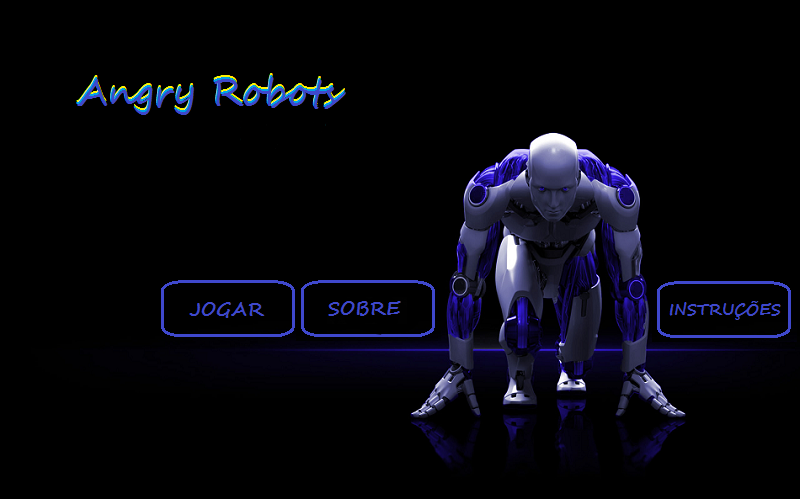
\includegraphics[scale=0.4]{menu.png}
\caption{Versão beta do jogo, com design teste.}
\end{figure}

\vspace{0.5cm}

\begin{figure}[!htb]
\centering
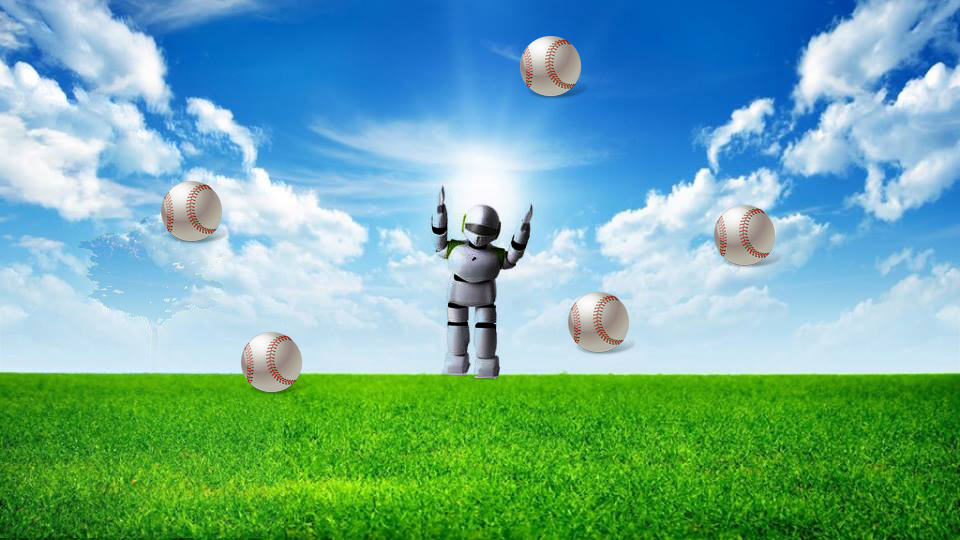
\includegraphics[scale=0.3]{fundo.jpg}
\caption{Imagem do jogo funcionando}
\end{figure}


\section*{Considerações Finais}

O rastreamento é o ponto mais difícil, pois alguns fatores atrapalharam o desenvolvimento do mesmo, um deles foi a iluminação, pois devido a ela, a imagem pode ser ofuscada ou obscurecida demais, porém o HSV permitiu que a iluminação fosse ignorada, pois este algoritmo converte toda a imagem para cinza, e trata a variação da luminosidade, deste modo o usuário poderá jogar com uma camiseta azul por exemplo, sem afetar o rastreamento.



\section*{Bibliografia}

http://labdegaragem.com/profiles/blog/list?tag=rob\%C3\%B3tica \\
http://labdegaragem.com/profiles/blog/list?tag=rob\%C3\%B4 \\
http://www.techtudo.com.br/noticias/noticia/2012/02/top-10-jogos-com-robos-gigantes.html \\
http://www.di.ubi.pt/~agomes/cg/teoricas/06-iluminacao.pdf \\
http://sidigicor.blogspot.com.br/2011/02/modelo-hsv.html \\
http://www.ufrgs.br/engcart/PDASR/formcor.html


\end{document}k